%%%%%%%%%%%%%%%%%%%%%%%%%%%%%%%%%%%%%%%%%%%%%%%%%%%%%%%%%%%%%%%
%
% Welcome to writeLaTeX --- just edit your LaTeX on the left,
% and we'll compile it for you on the right. If you give
% someone the link to this page, they can edit at the same
% time. See the help menu above for more info. Enjoy!
%
%%%%%%%%%%%%%%%%%%%%%%%%%%%%%%%%%%%%%%%%%%%%%%%%%%%%%%%%%%%%%%%

% --------------------------------------------------------------
% This is all preamble stuff that you don't have to worry about.
% Head down to where it says "Start here"
% --------------------------------------------------------------
 
\documentclass[12pt]{article}
 
\usepackage[margin=1in]{geometry}
\usepackage{amsmath,amsthm,amssymb}
\usepackage{hyperref}
\usepackage{enumitem}

\usepackage{listings}
\usepackage{xcolor}
\usepackage{graphicx}
\graphicspath{{./images/}}

%New colors defined below
\definecolor{codegreen}{rgb}{0,0.6,0}
\definecolor{codegray}{rgb}{0.5,0.5,0.5}
\definecolor{codepurple}{rgb}{0.58,0,0.82}
\definecolor{backcolour}{rgb}{0.95,0.95,0.92}

%Code listing style named "mystyle"
\lstdefinestyle{mystyle}{
  backgroundcolor=\color{backcolour}, commentstyle=\color{codegreen},
  keywordstyle=\color{magenta},
  numberstyle=\tiny\color{codegray},
  stringstyle=\color{codepurple},
  basicstyle=\ttfamily\footnotesize,
  breakatwhitespace=false,         
  breaklines=true,                 
  captionpos=b,                    
  keepspaces=true,                 
  numbers=left,                    
  numbersep=5pt,                  
  showspaces=false,                
  showstringspaces=false,
  showtabs=false,                  
  tabsize=2
}

%"mystyle" code listing set
\lstset{style=mystyle}

 
\newcommand{\N}{\mathbb{N}}
\newcommand{\Z}{\mathbb{Z}}
 
\newenvironment{theorem}[2][Theorem]{\begin{trivlist}
\item[\hskip \labelsep {\bfseries #1}\hskip \labelsep {\bfseries #2.}]}{\end{trivlist}}
\newenvironment{lemma}[2][Lemma]{\begin{trivlist}
\item[\hskip \labelsep {\bfseries #1}\hskip \labelsep {\bfseries #2.}]}{\end{trivlist}}
\newenvironment{exercise}[2][Exercise]{\begin{trivlist}
\item[\hskip \labelsep {\bfseries #1}\hskip \labelsep {\bfseries #2.}]}{\end{trivlist}}
\newenvironment{problem}[2][Problem]{\begin{trivlist}
\item[\hskip \labelsep {\bfseries #1}\hskip \labelsep {\bfseries #2.}]}{\end{trivlist}}
\newenvironment{question}[2][Question]{\begin{trivlist}
\item[\hskip \labelsep {\bfseries #1}\hskip \labelsep {\bfseries #2.}]}{\end{trivlist}}
\newenvironment{corollary}[2][Corollary]{\begin{trivlist}
\item[\hskip \labelsep {\bfseries #1}\hskip \labelsep {\bfseries #2.}]}{\end{trivlist}}

\newenvironment{solution}{\begin{proof}[Solution]}{\end{proof}}
 
\begin{document}
 
% --------------------------------------------------------------
%                         Start here
% --------------------------------------------------------------
 
\title{Homework 2}%replace X with the appropriate number
\author{Mengxiang Jiang\\ %replace with your name
CSEN 5322 Operating Systems} %if necessary, replace with your course title
 
\maketitle
 
\begin{problem}{1} %You can use theorem, exercise, problem, or question here.  Modify x.yz to be whatever number you are proving
Using figures describe RAID 6 in details. You are allowed to use Internet.
Proper citation must be provided.\\\\
RAID 6 uses block-level striping with distributed parity, like RAID 5.
However, there is an additional parity block distributed across all the member disks($D_p$, $E_q$ for Disk 0, $C_p$, $D_q$ for Disk 1, etc.).
The location of the parity blocks with respect to the data blocks can vary and the figure below is just one possible layout.
Read performance for RAID 6 is not negatively impacted by the second parity block compared to RAID 5, 
but writes are due to the additional overhead of not just the blocks but the parity calculations. 
The tradeoff for this performance penalty is that the system is more redundant, 
preserving data in case of more than one disk failure while RAID 5 only allows one.
\begin{figure}[ht]
    \centering
    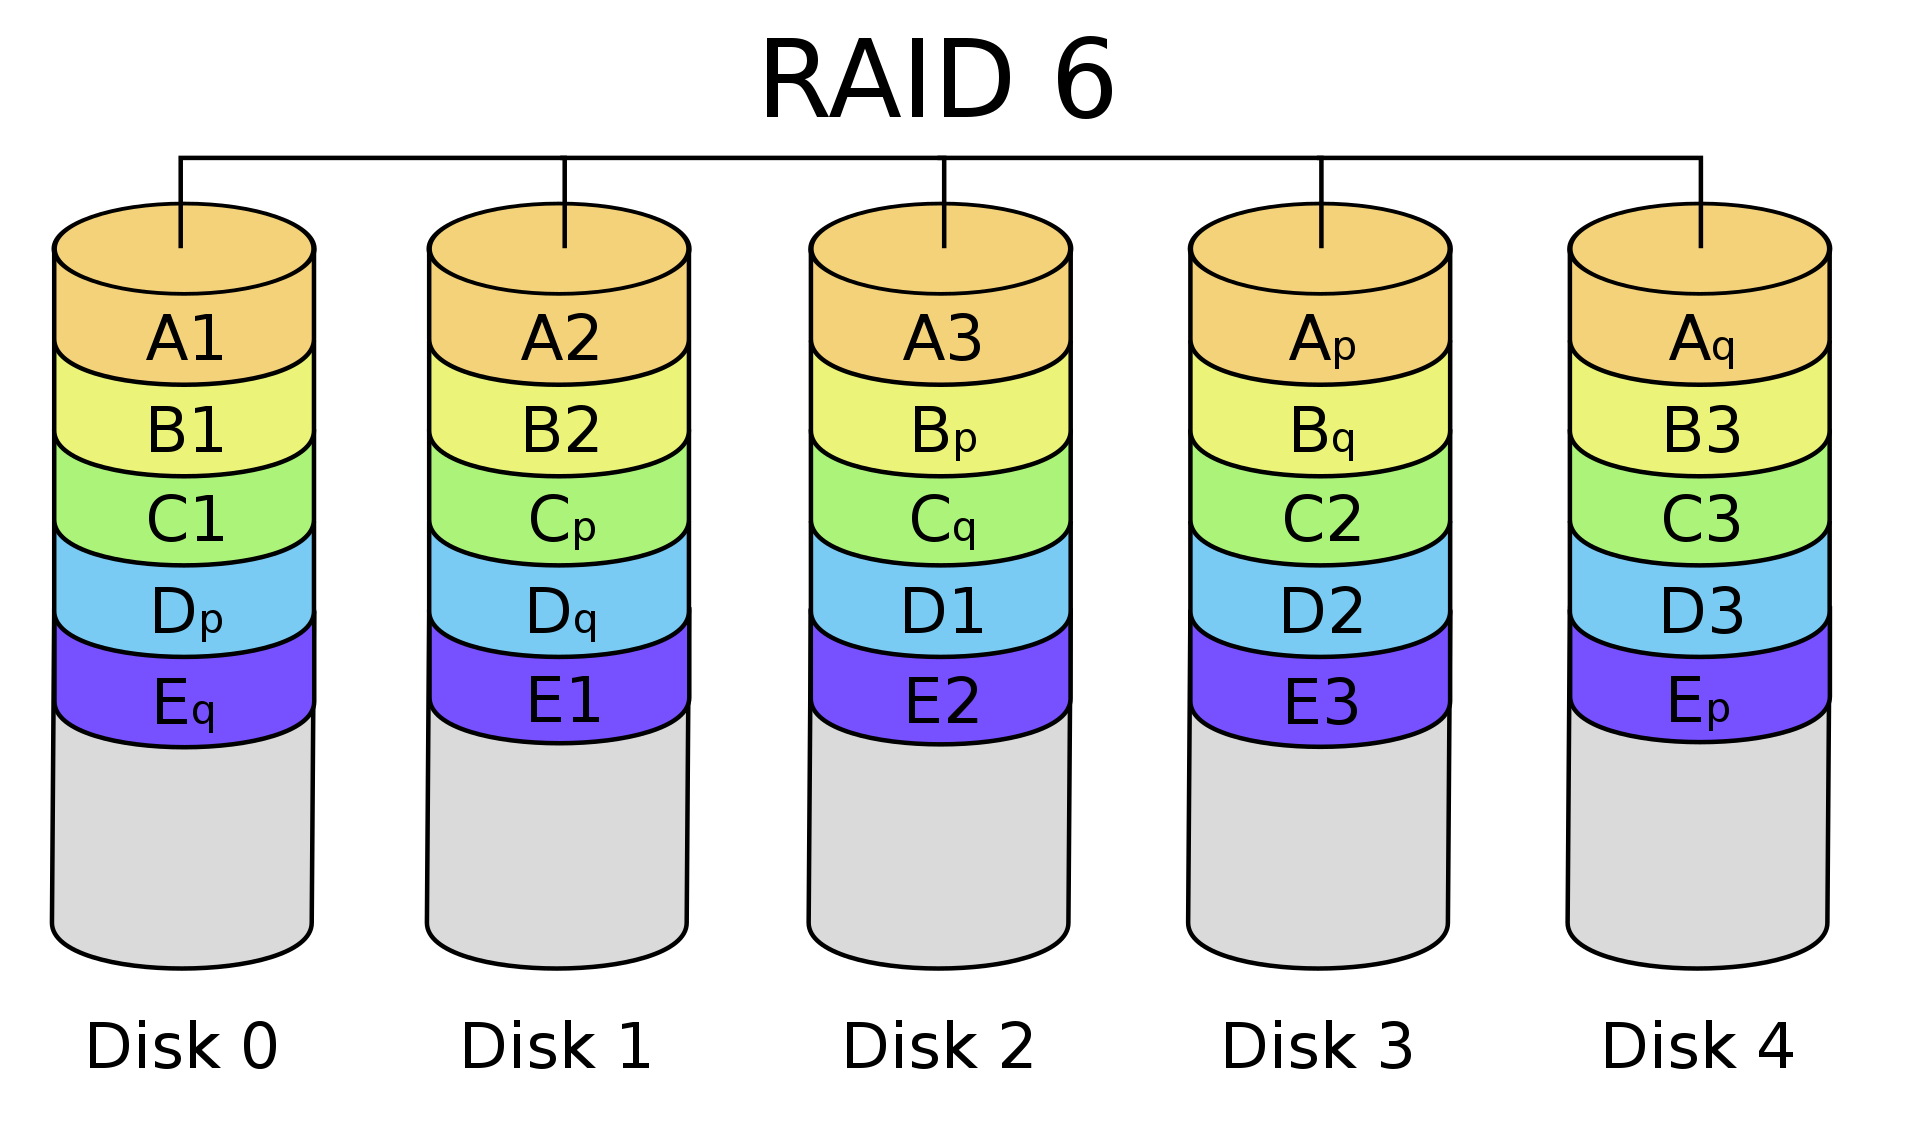
\includegraphics[width=\textwidth]{raid6}
\end{figure}
\\From \url{https://en.wikipedia.org/wiki/Standard_RAID_levels}
\end{problem}
\pagebreak
\begin{problem}{2}
Suppose that a machine has 42-bit virtual addresses and 32-bit physical
addresses.
\begin{enumerate}[label=\{\alph*\}]
    \item How much RAM can the machine support (each byte of RAM must be addressable)?\\
    Since the amount of memory that a machine can support only depends on the physical address, it is $2^{32}$ or 4 GB of RAM.
    \item What is the largest virtual address space that can be supported for a process?\\
    The largest virtual address space supported is $2^{42}$ or 4 TB. 
    \item If pages are 2 KB, how many entries must be in a single-level page table?\\
    2 KB pages require 11 bits, so there are $42 - 11 = 31$ bits left for entries. That is $2^{31}$ or roughly 2 billion entries.
    \item If pages are 2 KB and we have a two-level page table where the first level is indexed by 15 bits, 
    then how many entries does the first level page table have?\\
    Since the first level is indexed by 15 bits, there are $2^{15}$ or around 32 thousand entries.
    \item With the same setup as part \{d\}, how many entries are in each second-level page table?\\
    2 KB pages require 11 bits of offset, and we used 15 bits for the first level, 
    so $42-11-15=16$ are left for the second level. This is $2^{16}$ or around 65 thousand entries.
    \item What is the advantage of using a two-level page table over single-level page table?\\
    Two levels means the number of pages in the page table that need to be in memory is much fewer than a single level.
    This is because most processes will only need the top level page table, one instruction page, and one data page 
    instead of the entire page table for a single level.
\end{enumerate}
\end{problem}
\pagebreak
\begin{problem}{3}
    Base64 and mount
\begin{enumerate}[label=(\alph*)]
    \item What is Base64? Show at least one application of Base64.\\
    If we're going by math conventions, Base64 would be a number system with 64 different digits 
    (0, 1, ..., ?) where $10_{64}$ = $64_{10}$. 
    In computer science usage, it refers to a group of binary-to-text encoding schemes
    that represent data using 4 6-bit ($2^{6} = 64$) Base64 digits.\\\\
    One application is Multipurpose Internet Mail Extensions (MIME) Base64 for Privacy-enhanced Electronic Mail (PEM) protocol:\\\\
    Given a sentence to be encoded: Many hands make light work.\\
    The Base64 encoding is: TWFueSBoYW5kcyBtYWtlIGxpZ2h0IHdvcmsu\\
    For the first three characters, $M$, $a$, and $n$, the ASCII values are 77, 97, and 110 respectively.
    These are converted to the binary values 01001101, 01100001, and 01101110, which when concatenated
    into a single 24 bit string, produces 010011010110000101101110. Split this into 4 groups of 6 bits, we get
    010011, 010110, 000101, 101110, which corresponds with $T$, $W$, $F$, and $u$ in Base64.\\
    From \url{https://en.wikipedia.org/wiki/Base64}
    \item What does $mount$ command do in UNIX? Explain with example.\\
    The $mount$ command is used to associate additional file systems such
    as CDs, USB drives, external hard drives, etc. to the root file system. 
    The reason why this is necessary is because in UNIX, 
    you cannot specify path names to be prefixed by a drive name. 
    Therefore you have to attach the additional file system to some directory 
    on the root file system, which is done using $mount$. Suppose you inserted a CD 
    into your optical drive, and you're using UNIX. Suppose the operating system did not 
    automatically $mount$ the file system of the CD for you, then to access the files 
    on the CD, you would use $mount$ to specify a directory for the CD's file system to reside
    such as $/b$.
    After that you can then access the files on the CD at the directory $/b$ such as the file $/b/x$.
    However, if the directory was not empty before $mount$, you would not be able to access those files 
    until you have $umount$ the CD.
\end{enumerate}
\end{problem}
\pagebreak
\begin{problem}{4}
Our CPU is currently idle and the current time is labeled time 0. Four
processes arrive to the ready queue at the following times and with the following required
run time:\\\\
\begin{tabular}{|c|c|c|} 
    \hline
    Process & Arrival Time & Run Time\\
    \hline
    A & 0 & 9\\
    B & 1 & 28\\
    C & 2 & 7\\
    D & 3 & 3\\
    \hline
\end{tabular}
\\\\Simulate the process scheduling and execution under the FCFS, SJF, and SRTN scheduling
algorithms. Indicate each scheduling decision, and calculate the turnaround time for each
process. Also calculate the average turnaround time for each scheduling algorithm.\\\\
FCFS:\\
\begin{tabular}{|c|c|c|c|} 
    \hline
    A finished at 9 & B finished at 37 & C finished at 44 & D finished at 47 \\
    \hline
\end{tabular}
$$\text{Average turnaround time = }\frac{9+37+44+47}{4} = 34.25$$
SJF:\\
\begin{tabular}{|c|c|c|c|} 
    \hline
    A finished at 9 & D finished at 12 & C finished at 19 & B finished at 47 \\
    \hline
\end{tabular}
$$\text{Average turnaround time = }\frac{9+12+19+47}{4} = 21.75$$
SRTN:\\
\begin{tabular}{|c|c|c|c|c|} 
    \hline
    A preempted by D at 3& D finished at 6 & A finished at 12& C finished at 19 & B finished at 47 \\
    \hline
\end{tabular}
$$\text{Average turnaround time = }\frac{6+12+19+47}{4} = 21$$
\end{problem}
\pagebreak
\begin{problem}{5}
At the end of chapter 2, we studied a solution to the readers and writers problem,
given below: 

\begin{lstlisting}[language=C, caption=readers-preference]
typedef int semaphore;          /* use your imagination */
semaphore mutex = 1;            /* controls access to rc */
semaphore db = 1;               /* controls access to the database */
int rc = 0;                     /* # of processes reading or wanting to */

void reader(void)
{
    while (TRUE) {                  /* repeat forever */
        down(&mutex);               /* get exclusive access to rc */
        rc = rc + 1;                /* one reader more now */
        if (rc == 1) down(&db);     /* if this is the first reader ... */
        up(&mutex);                 /* release exclusive access to rc */
        read_data_base();           /* access the data */
        down(&mutex);               /* get exclusive access to rc */
        rc = rc - 1;                /* one reader fewer now */
        if (rc == 0) up(&db);       /* if this is the last reader ... */
        up(&mutex);                 /* release exclusive access to rc */
        use_data_read();            /* noncritical region */
    }
}

void writer(void)
{
    while (TRUE) {                  /* repeat forever */
        think_up_data();            /* noncritical region */
        down(&db);                  /* get exclusive access */
        write_data_base();          /* update the data */
        up(&db);                    /* release exclusive access */
    }
}
\end{lstlisting}
In this solution, as long as one reader is having the resource any new reader can get access to the
resource. Thus, the writer will have to wait for an opportunity for all the readers to release the
resource to have an exclusive access to that resource.

Here, you have to modify the solution so that once the writer expresses interest to have the
resource, no new reader will be granted access to the resource and the new reader(s) will have to
wait for the writer to avail the resources exclusively and then to release the resource. Of course,
after expressing interest the writer will also have to wait for all the existing resource-occupying-reader(s) to be done and release the resource. 
\end{problem}
\pagebreak
\begin{lstlisting}[language=C, caption=writers-preference]
typedef int semaphore;          /* use your imagination */
semaphore rmutex = 1;           /* controls access to rc */
semaphore wmutex = 1;           /* controls access to wc */
semaphore readTry = 1;          /* controls access to trying to read */
semaphore db = 1;               /* controls access to the database */
int rc = 0;                     /* # of processes reading or wanting to */
int wc = 0;                     /* # of processes writing or wanting to */

void reader(void)
{
    while (TRUE) {                  /* repeat forever */
        down(&readTry);             /* indicate reader trying to read */
        down(&rmutex);              /* get exclusive access to rc */
        rc = rc + 1;                /* one reader more now */
        if (rc == 1) down(&db);     /* if this is the first reader ... */
        up(&rmutex);                /* release exclusive access to rc */
        up(&readTry);               /* indicate reader done trying */
        read_data_base();           /* access the data */
        down(&rmutex);              /* get exclusive access to rc */
        rc = rc - 1;                /* one reader fewer now */
        if (rc == 0) up(&db);       /* if this is the last reader ... */
        up(&rmutex);                /* release exclusive access to rc */
        use_data_read();            /* noncritical region */
    }
}

void writer(void)
{
    while (TRUE) {                  /* repeat forever */
        think_up_data();            /* noncritical region */
        down(&wmutex);              /* get exclusive access to wc */
        wc = wc + 1;                /* one more writer now */
        if (wc == 1) down(&readTry);/* lock readers out of trying */
        up(&wmutex);                /* release exclusive access to wc */
        down(&db);                  /* get exclusive access */
        write_data_base();          /* update the data */
        up(&db);                    /* release exclusive access */
        down(&wmutex);              /* get exclusive access to wc */
        wc = wc - 1;                /* one fewer writer now */
        if (wc == 0) up(&readTry);  /* allow readers to try again */
        up(&wmutex);                /* release exclusive access to wc */
    }
}
\end{lstlisting}
\bibliographystyle{plain}
\bibliography{refs}


% --------------------------------------------------------------
%     You don't have to mess with anything below this line.
% --------------------------------------------------------------
 
\end{document}